\chapter{Project Management}
\pageauthor{Helena Adam}
\section{Scrum}
\subsection{Description of Scrum}
Scrum is an iterative and incremental agile process used to develop software. The team had to organize itself by taking the tasks from the scrum board.

At the beginning of developing the product, the project goals got divided into sprints. To have an overview over the whole project, the so called scrum meetings were held. During these scrum meetings, done tasks and what's left to do, got discussed. Those discussions can be held daily and help to see the process of the project.

Three different roles are represented in Scrum. Firstly, the development team. They are responsible for the programming part of the software. Secondly, the product owner. He provides the user stories the development  team has to do. Moreover, to keep the customer satisfied, he makes sure that the software has included everything the customer requested. Last but not least, the Scrum master. Disturbances can delay the milestones deadlines. To prohibit this, he makes sure that the development team can work efficient without the project managers or the customers interference.

\subsection{Why we have chosen Scrum}
As already mentioned above, scrum is agile because of the sprints. Basically, it means that there is no problem in changing or adding sprints in the current tasks without a delay. We have already had a good experience with Scrum in the 3rd grade. So, we already knew that Scrum works really good with managing changes. As it was our first “big” project and we had no idea how often we could change our project, we decided on Scrum.
\newpage
\section{Project Organization Chart}
The following diagram shows the structure of the organization. It pictures who was involved, what their position in the project was and their relation to each other. 

Our contact person for our diploma-thesis was DI Dominik Fuchshofer. He is the \gls{ceo} of the company Sunlime IT Services GmbH, we created our work for. Our two supervisors DI Dr. Wolfgang Pölzleitner and DI Florian Schreiber took care of the progress we made. The members of our project team are Helena Adam, Claudio Knapp, Laura Rössl and Paul Zwölfer. Everyone communicated with the employer on its own, over Hangouts.
\begin{center}
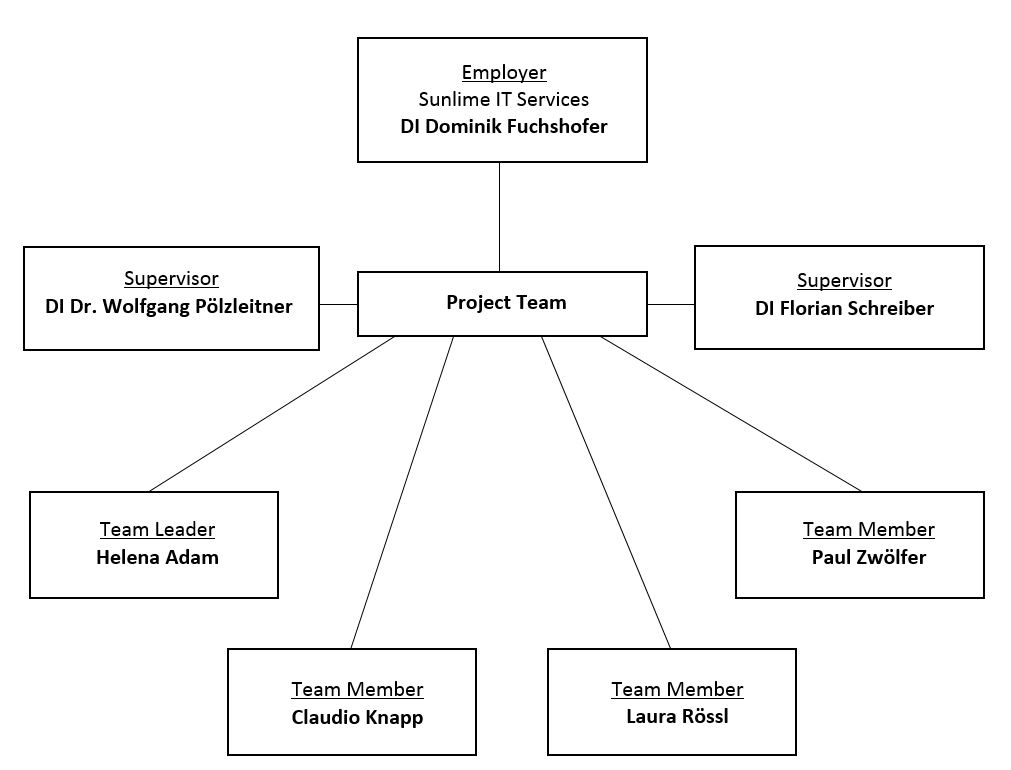
\includegraphics[width=0.8\textwidth] {bilder/projectdiagram}
\end{center}
\clearpageauthor
\newpage
\section{Milestones}
\pageauthor{Helena Adam}
Milestones are tools for the project management to schedule the project. The present work gets divided into some parts. Then, it gets defined until when a part has to be done. This tool is used to avoid bigger delays in this project.\newline

In the chart below it is visible into which parts we have divided our diploma-thesis and the date until it was due.\newline
\begin{center}
\begin{tabular}{p{5cm}p{5cm}}
\toprule
\textbf{Milestones} & \textbf{Deadline} \\
\midrule
Competitor analysis & July 10, 2015 \\
Wireframing & July 31, 2015 \\
Designing of data & November 24, 2015 \\
Functioning software & January 12, 2016 \\
Hardware prototype & February 16, 2016 \\
Bug fixing & February 23, 2016 \\
Documentation & \today \\
\bottomrule
\end{tabular}
\end{center}
\newpage
\section{Working Hours}
Here you can see a listing of our working hours and how much time we spent on different tasks. You can see in the following table that we spent the most hours on documentation of the diploma thesis. The main reason for this is the technology LaTeX we used. \newline
\begin{center}
\begin{tabular}{p{5cm}p{2cm}}
\toprule
\textbf{Type} & \textbf{Hours} \\
\midrule
Administration & 194,05 \\
Designing & 7 \\
Data design & 43 \\
Documentation & 225,7 \\
Programming & 179,75 \\
Research & 85 \\
Raspberry Pi & 140 \\
Testing & 18 \\
UML Diagrams & 14 \\
Wireframing & 81 \\
\bottomrule
\end{tabular}
\end{center}
\clearpageauthor